\chapter{ILD detector simulation studies}

Simulation of detector response is an essential part in high energy physics experiment. In Early stage of a project, simulations are done in order to explore and understand the possibilities of a detector design as well as its limitations. Simulation can be use as a way to determine requirements of an experiment to reach certain goals. During data-taking and afterwards, simulations are used model physics processes to compare  the expected value from theory to a measured value for various processes.
In this chapter, software tools will be briefly introduced. The \ilcsoft framework used for this analysis will be described in \ref{}. The chain starts by the simulation of single kaons $(K^{0}_{L})$ interaction with the ILD detector model based on \geant. Then simulated events undergoes the full chain reconstruction as explained in \ref{}. The procedure of the analysis (based on Marlin) and its conclusions will be presented in \ref{}.
Finally, a benchmark of a fast simulation software (SGV) against the ILD full simulation will be described in \ref{}, particularly focussing on particle-flow performance aspects.

\section{Simulation and software framework}

\subsection{\ilcsoft software framework}

Various tools developed by the Linear Collider community is regrouped in a common software framework called \ilcsoft \cite{ILCSoftPortal}. It provides a complete framework that can be used for Monte-Carlo studies and experiments. As an example, physics studies, ILD detector optimisation and performance for the ILC are performed under the \ilcsoft framework.

Most of the tools in the framework use an Event Data Model (EMD) named Linear Collider I/O (\lcio) which provides a reliable and performant solution for simulation and analysis studies \cite{Gaede:2003ip}. With this tool, various detector concepts and analysis can be shared.

The \ilcsoft framework provides a modular \cpp framework named \marlin for reconstruction and analysis of physics events \cite{Gaede:2006pj}. \marlin uses \lcio seamlessly and is configured using XML steering files. \marlin enables users to develop custom modules for their own and run it along other already existing modules.

The reconstruction and analysis tools used in this analysis are mostly part of \ilcsoft. For this thesis, \ilcsoft v01-17-11 was used for simulation, reconstruction and analysis.

\subsection{ILD Detector Simulation}

The following analysis is using one of the generic ILD detector model (ILD\_o1\_v05) as describe in \ref{} within the \mokka framework. Many other models are also considered for ILD as shown in Table \ref{ILDOptions}. \mokka is a front-end to \geant and provides a realistic geometry of the ILD detector. The \mokka version used is v08-05 and the \geant version is 10.01.
The simulation is performed by simply using the particle gun provided in \geant to shoot particles ($\pi^{-}$ or $K^{0}_{L}$) in different regions of the detector by randomly variating the angles $\theta$ and $\phi$ of the gun. To model hadronic showers, the QGSP\_BERT physics list was used. The output of the simulation provides a lcio file containing collections of the tracking hits and simulated calorimeter hits. This file is then reconstructed within \marlin.

\begin{table}[t]
  \centering
  \caption{Considered ILD detector options.} \label{ILDOptions}
  \begin{tabular}{|c|c|c|}
    \hline
    Option & ECAL Technology & HCAL Technology \\
    \hline
    ILD\_o1\_v05 & SiW-ECAL & AHCAL \\
    ILD\_o2\_v05 & SiW-ECAL & SDHCAL \\
    ILD\_o3\_v05 & Sc-ECAL & AHCAL \\
    \hline
  \end{tabular}
\end{table}

\section{Reconstruction chain}

The reconstruction is done on simulated data in order to implement detector effects. For example, calorimeter hits need to be digitized by implementing threshold and readout effects.

\subsection{Tracking}

The tracking reconstruction is performed on each individual tracking detector. Track segments are identified by pattern recognition algorithms.

Track fitting is performed using the track segments with an inversed Kalman filter to identify trajectories of charged particles. Each tracks contains origin, direction, charge and momentum of the particle \cite{Fruhwirth:1987fm}.

\subsection{Calorimeter digitization}

The calorimeter digitisation is performed on simulated calorimeter hits as part of ILDCaloDigi processor \cite{Jeans2015}. It takes account for threshold effect from the electronics, sampling fraction of the calorimeter and the readout technology used. In the considered model of ILD, the SiW-ECAL and AHCAL are used.

In both cases, it uses a silicon-pixel based technology. The digitisation then takes into account the finite number of pixels that can be fired as well as the statistical fluctuations related to pixel readout \cite{Hartbrich:2016bbz}.

Concerning time, it uses a simple digitisation. For a simulated hit, all contributions are looped over and only adds contributions under a certain timing cut (default is \SI{100}{\ns}). This modelisation of timing is very simplified as in reality the electronics are shaping the signal with a certain shapping time and register the time of the first contribution over the threshold (default is 0.5 MIP) \ref{}.

\subsection{Pandora PFA}

PandoraPFA \cite{Thomson:2009rp} is the Particle Flow algorithm used for Linear Colliders as explained in \ref{}. It uses as input tracks and calorimeter hits to form Particle Flow Objects (PFO). It uses a complex multi-stage process but basically, calorimeter hits are clustered and associated to tracks (if any) then the energy of a cluster can be corrected to improve the energy resolution. If the right criterium are matched, it forms a PFO which contains information about the reconstructed objects.

\section{Influence of time cuts on hadronic showers}

In this section, a study of timing cuts on hadronic shower is performed. The goal of this study is to assess the influence of timing cuts on the properties of hadronics showers as for example the width of the shower as well as the needed time resolution. The study will be divided in 2 parts, the first part assuming a perfect time resolution and the second part assuming time resolution for different cases.

\subsection{Modification of timing window in ILDCaloDigi}

Timing of hits is registered in a very simplyfied way as explained in \ref{}. The modification of the time window (ranging from 1 ns to 100 ns) is performed during the reconstruction for different simulated $K^{0}_{L}$ energies (ranging from 5 to 90 GeV).

\subsection{Effects of calibration constants and Pandora constants}

\begin{figure}
  \centering
  \begin{subfigure}[t]{0.45\textwidth}
    \centering
    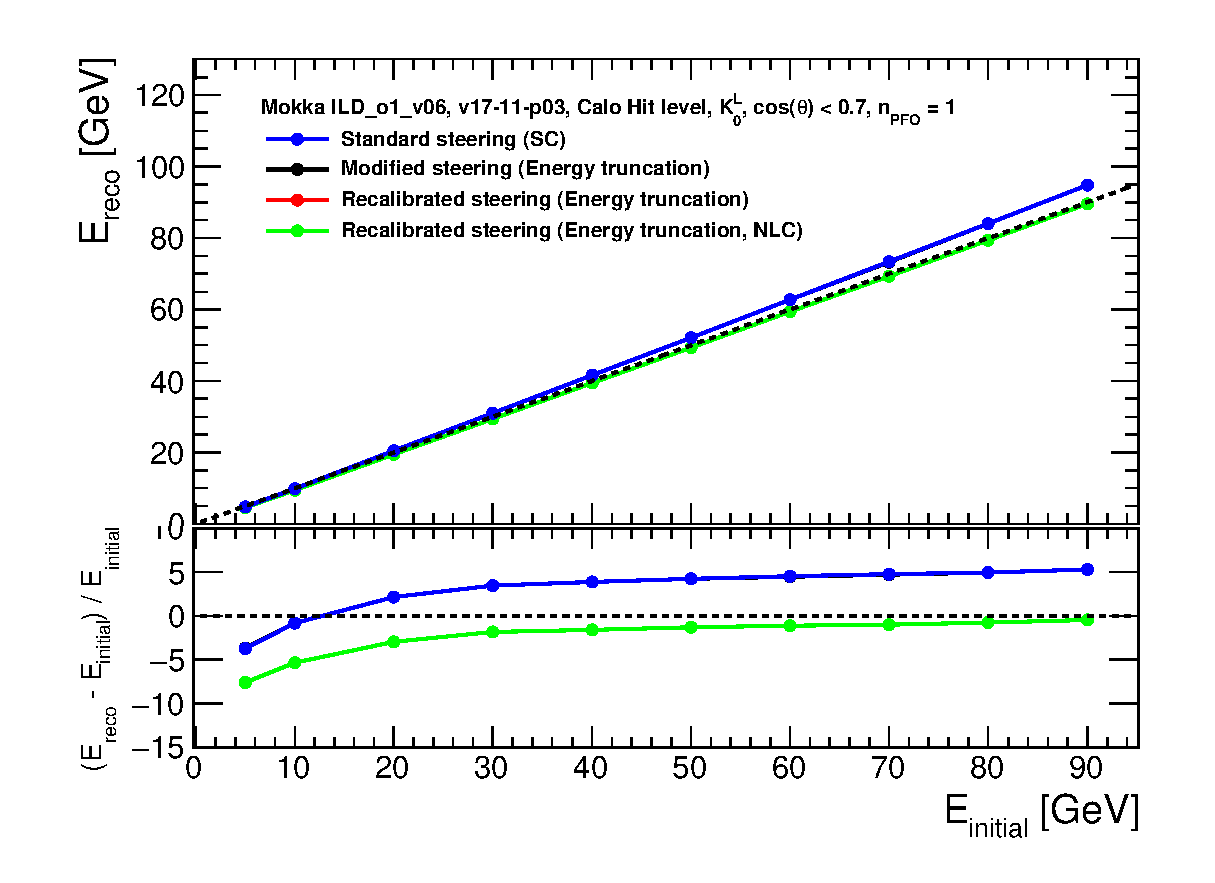
\includegraphics[width=\linewidth]{chap6/fig_TimingILD/Comparison_linearity_Curves_Hits}
    \caption{Linearity curve} \label{fig:linhits}
  \end{subfigure}
  \hfill
  \begin{subfigure}[t]{0.45\textwidth}
    \centering
    \includegraphics[width=\linewidth]{chap6/fig_TimingILD/Comparison_resolution_Curves_Hits}
    \caption{Resolution curve} \label{fig:resohits}
  \end{subfigure}
  \caption{\subref{fig:linhits}) The top plot shows the mean reconstructed energy $E_{reco}$ for 5 to 90 GeV $K^{0}_{L}$ function of the simulated energy $E_{initial}$ for different constant parameters used in the reconstruction. The bottom plot shows the relative difference of the different curve to the line $x = y$. \subref{fig:resohits}) The plot shows the relative resolution $RMS_{90}/Mean_{90}$ for different constant parameters used in the reconstruction function of the energy. The blue curve uses the standard calibration, the black curve uses a modified set of parameters using energy truncation and no SC, the red curve uses constant parameters after recalibration and the green curve uses the same parameters as the red curve with non-linearity correction. The error bars represent statistical uncertainties.}
\end{figure}

% \begin{figure}[!h]
%   \centering
%   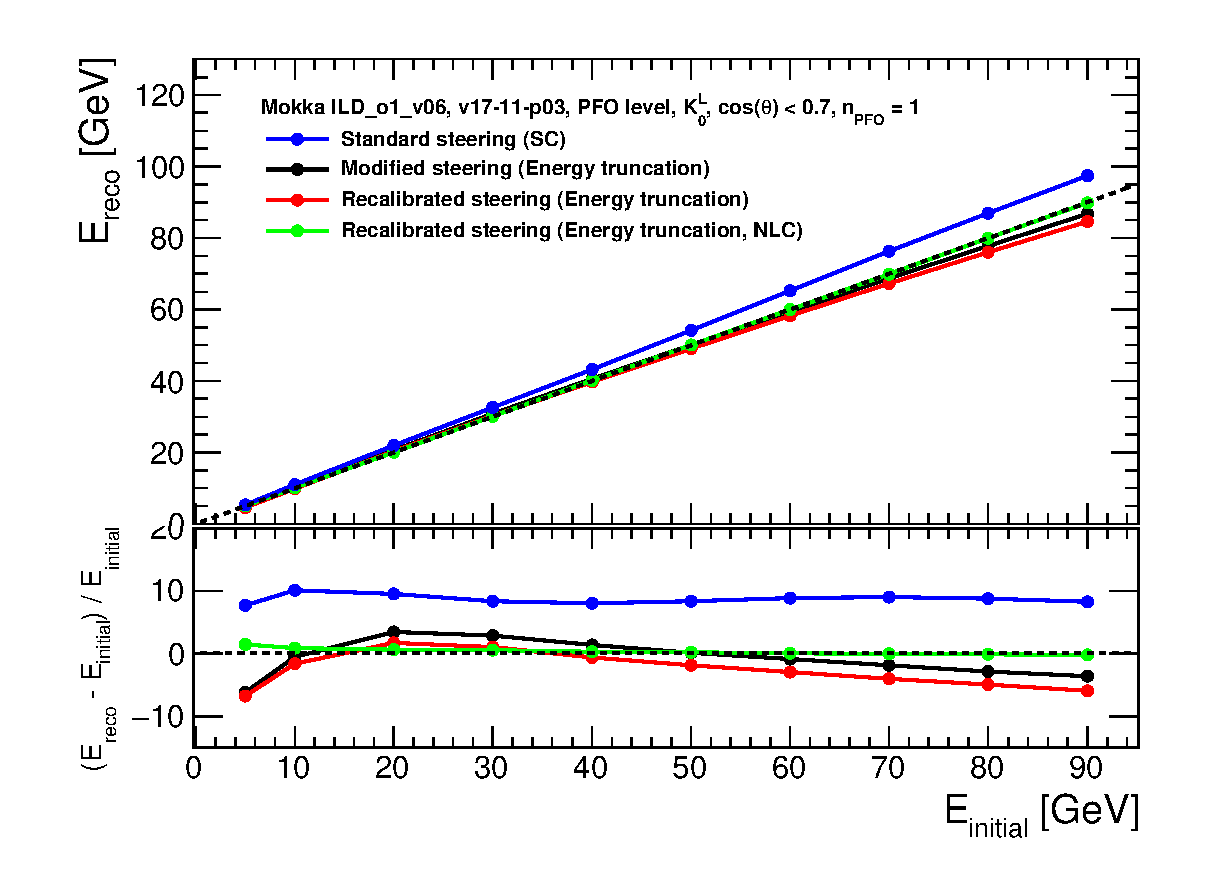
\includegraphics[scale=0.5]{chap6/fig_TimingILD/Comparison_linearity_Curves_PFO}
%   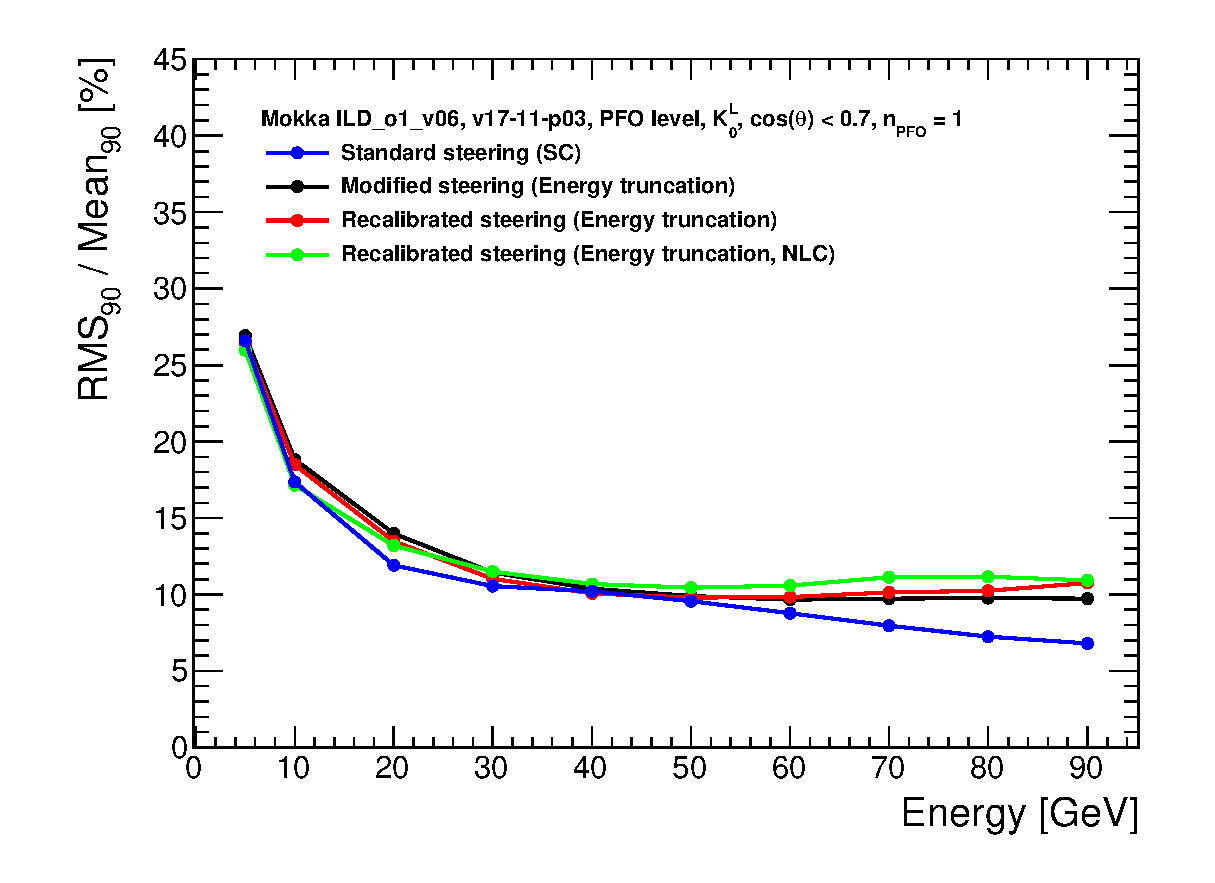
\includegraphics[scale=0.5]{chap6/fig_TimingILD/Comparison_resolution_Curves_PFO}
%   \caption{title}
% \end{figure}

\subsection{Timing cut Effects on hadronic showers}

\section{Benchmarking of fast simulation}

\subsection{SGV: fast simulation software}
\subsection{Particle Flow parametrisation}
\subsection{Benchmarking against full ILD Simulation}
